\chapter{Dataset}
\label{ch:dataset}
This chapter discusses the dataset used in our work. We use the \gls{scid} dataset \cite{ni_esim_2017}\footnote{The dataset can be downloaded here: https://eezkni.github.io/publications/ESIM.html.}.
The important characteristics of the dataset are text content on screenshots, different distortion levels and \gls{mos} values for each image.

- authors name it mos, but it should be dmos, because double stimulus \cite{mos_dmos_1993}
- still use mos for rest of work

We did not find any other dataset with the same characteristics.
Other screen content datasets are mentioned in \cite{iqa_survey_2020}, but we either were not able to access them or they did not contain enough text based images.

\section{Overview}
\label{sec:dataset_overview}
An overview of the 40 reference images of the dataset can be seen in \autoref{fig:dataset_overview}.

\begin{figure}[h]
    \centering
    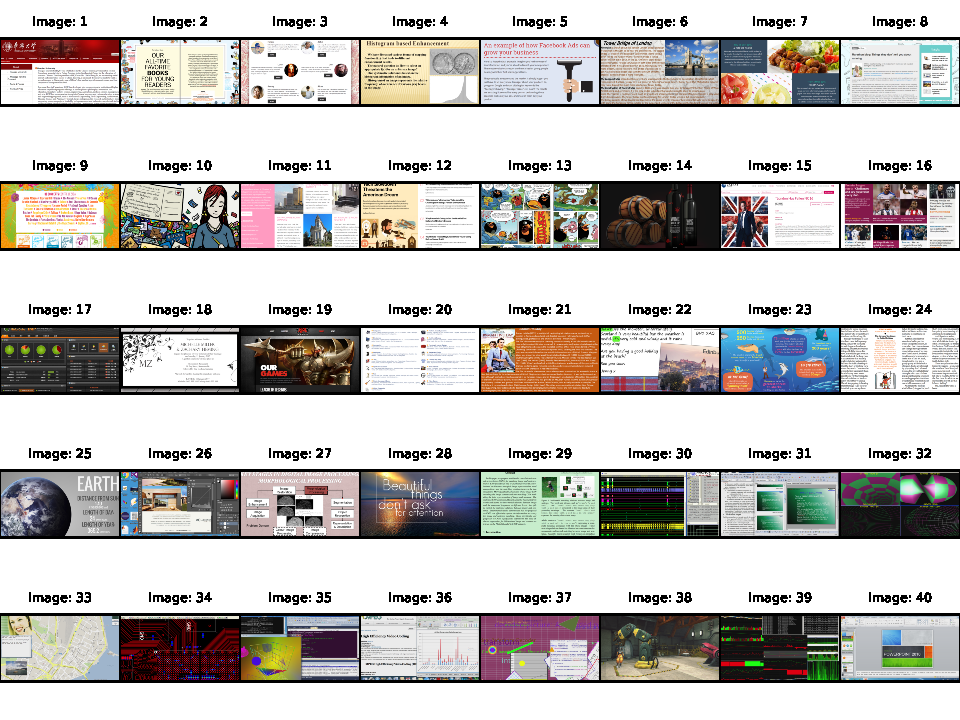
\includegraphics[width=\textwidth]{reference_images}
    \caption{Overview of the dataset.}
    \label{fig:dataset_overview}
\end{figure}

Additionally, the dataset contains 1800 distorted images.
They are distorted with 9 different distortion types, each with 5 different distortion levels.

\section{Distortion types}
\label{sec:dataset_distortion_types}

In this section we will discuss the different distortion types used in the dataset.
The nine different distortion types can be seen in \autoref{fig:distortion_types}, applied to the image in \autoref{fig:img29}.

\begin{table}[h]
\centering
\caption{Distortion types used in the dataset.}
\begin{tabular}{|p{6cm}|l|p{6cm}|}
\hline
\textbf{Distortion Type} & \textbf{Abbreviation} & \textbf{Description} \\
\hline
Contrast Change & CC & Changes in the contrast of an image \\
\hline
Color Quantization with Dithering & CQD & Reduction of colors in an image using dithering \\
\hline
Color Saturation Change & CSC & Changes in the color saturation of an image \\
\hline
Gaussian Blur & GB & Blurring of an image using a Gaussian function \\
\hline
Gaussian Noise & GN & Addition of noise to an image using a Gaussian distribution \\
\hline
High Efficiency Video Coding-Screen Content Coding & HEVC-SCC & Video compression standard for screen content \\
\hline
Joint Photographic Experts Group & JPEG & Image compression standard \\
\hline
Joint Photographic Experts Group 2000 & JPEG2000 & Image compression standard \\
\hline
Motion Blur & MB & Blurring of an image due to movement \\
\hline
\end{tabular}
\label{tab:distortion_types}
\end{table}


\begin{figure}[h]
    \centering
    \begin{subfigure}[b]{0.3\textwidth}
        \includegraphics[width=\textwidth]{../../data/raw/scid/DistortedSCIs/SCI29_1_5.png}
        \caption{Gaussian Noise}
        \label{fig:distortion_type_1}
    \end{subfigure}
    \hfill
    \begin{subfigure}[b]{0.3\textwidth}
        \includegraphics[width=\textwidth]{../../data/raw/scid/DistortedSCIs/SCI29_2_5.png}
        \caption{Gaussian Blur}
        \label{fig:distortion_type_2}
    \end{subfigure}
    \hfill
    \begin{subfigure}[b]{0.3\textwidth}
        \includegraphics[width=\textwidth]{../../data/raw/scid/DistortedSCIs/SCI29_3_5.png}
        \caption{Motion Blur}
        \label{fig:distortion_type_3}
    \end{subfigure}
    \newline
    \begin{subfigure}[b]{0.3\textwidth}
        \includegraphics[width=\textwidth]{../../data/raw/scid/DistortedSCIs/SCI29_4_5.png}
        \caption{Contrast Change}
        \label{fig:distortion_type_4}
    \end{subfigure}
    \hfill
    \begin{subfigure}[b]{0.3\textwidth}
        \includegraphics[width=\textwidth]{../../data/raw/scid/DistortedSCIs/SCI29_5_5.png}
        \caption{JPEG Compression}
        \label{fig:distortion_type_5}
    \end{subfigure}
    \hfill
    \begin{subfigure}[b]{0.3\textwidth}
        \includegraphics[width=\textwidth]{../../data/raw/scid/DistortedSCIs/SCI29_6_5.png}
        \caption{JPEG2000 Compression}
        \label{fig:distortion_type_6}
    \end{subfigure}
    \newline
    \begin{subfigure}[b]{0.3\textwidth}
        \includegraphics[width=\textwidth]{../../data/raw/scid/DistortedSCIs/SCI29_7_5.png}
        \caption{Color Saturation Change}
        \label{fig:distortion_type_7}
    \end{subfigure}
    \hfill
    \begin{subfigure}[b]{0.3\textwidth}
        \includegraphics[width=\textwidth]{../../data/raw/scid/DistortedSCIs/SCI29_8_5.png}
        \caption{HEVC Screen Content Coding}
        \label{fig:distortion_type_8}
    \end{subfigure}
    \hfill
    \begin{subfigure}[b]{0.3\textwidth}
        \includegraphics[width=\textwidth]{../../data/raw/scid/DistortedSCIs/SCI29_9_5.png}
        \caption{Color Quantization with dithering}
        \label{fig:distortion_type_9}
    \end{subfigure}
    \caption{Distorted image 29 with 9 different distortion types and distortion level 5.}
    \label{fig:distortion_types}
\end{figure}

We can see, that the different distortion types have different effects on the text in the image.
Distortions like the contrast change don't affect the text much.
However, Gaussian noise or blur can make the text unreadable.
\section{Labeling}
\label{sec:dataset_labeling}

The dataset doesn't have any text labels.
Thus we labeled the dataset ourselves.
We typed the text on each image into a text file, starting on the top left and ending on the bottom right.
Our order of labeling was always dependent on the top left corner of a text element.
Thus if two paragraphs were side by side we always labeled the first line of the left paragraph first, then the first line of the right paragraph, then the second line of the left paragraph and so on.
This way we could ensure that we have a unifying representation of the text with regards to the two /gls{ocr} algorithms we used.
The algorithms have different modes for combining text elements, and thus produce differently connected paragraphs, if using the paragraph option.
To get a generalized result we use the option of raw text detection and text recognition to get the bounding boxes and the text.
We then use the bounding boxes to get the text in the correct order.

In \autoref{fig:ref29} we can see that it is sometimes difficult to say which text element is higher than another, especially if the text elements have different font sizes.
Thus we decided against using one of the \gls{ocr} algorithms to predict the text and then correct it to create the ground truth, to not introduce bias towards one of the algorithms with regard to the positions of the text elements.
We used the images, a ruler and our eyes to determine the correct order of the text elements.

- Select based on how hard to label
- Select based on how much text/objects
- very subjective
- different metric with IoU and CER combined might be helpful

- go through all the distortions and make hypothesis on how they affect the ocr, check for literature on this
- check later in evaluation if true/false
- mos vs dmos / single stimulus vs double stimulus

\begin{figure}
    \centering
    \includegraphics[width=\textwidth]{../../data/raw/scid/ReferenceSCIs/SCI29.png}
    \caption{Reference image 29.}
    \label{fig:ref29}
\end{figure}

\section{Analysis}
\label{sec:dataset_analysis}

In \autoref{fig:cer_vs_mos} the cer is plotted against the MOS.
It shows the \gls{cer} and \gls{mos} of all 1800 distorted images compared to their reference image.

\begin{figure}[h]
    \centering
    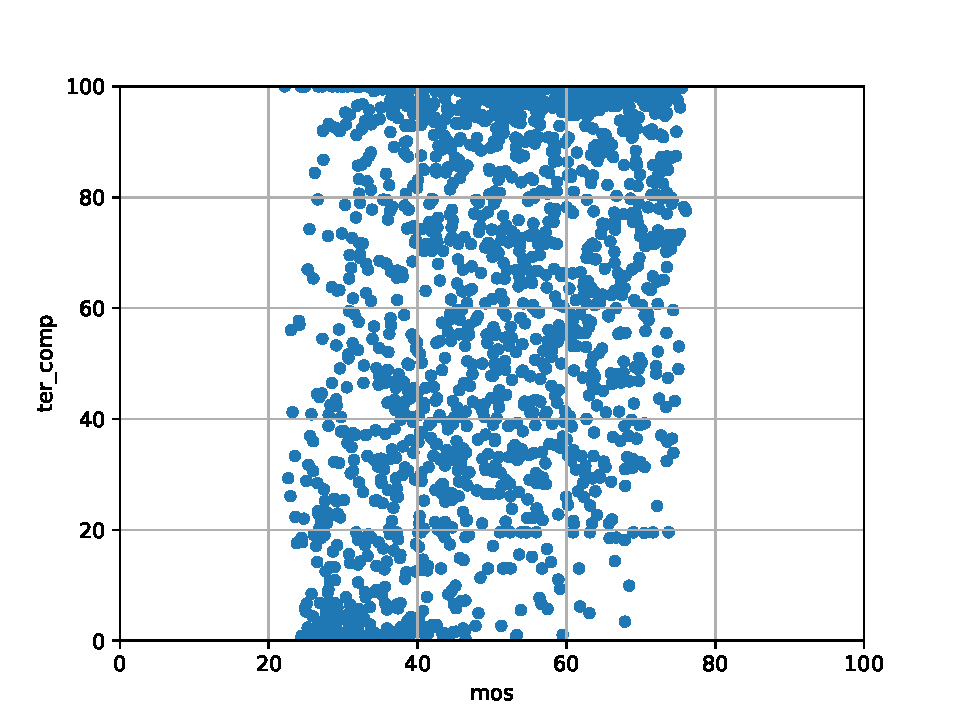
\includegraphics[width=\textwidth]{mosvster_all}
    \caption{\gls{cer} of all distorted images compared to their reference image plotted against the \gls{mos}.}
    \label{fig:cer_vs_mos}
\end{figure}

In \autoref{fig:cer_vs_mos_456} the \gls{cer} is plotted against the \gls{mos}.
We are only using a selection of images in this plot.
The images with the ID's $[1, 2, 3, 4, 5, 6, 7, 8, 11, 12, 15, 18, 20, 21, 24, 29]$ have their main focus on text, and have a relatively simple text structure.
Thus those images are used in experiments that involve the \gls{mos}.

- even if images have only one line of text, cer might still be a good metric, as distortion affects that line the same as it affects the whole image.
- so if mos is low because objects look bad, if cer is a good metric, it should be low as well, as the text is also affected by the distortion
- but distortions generally dont affect text the same as objects
- objective is more to check if cer is a good metric to simulate mos for readability of text
- although it might be less consistent
\begin{figure}[h]
    \centering
    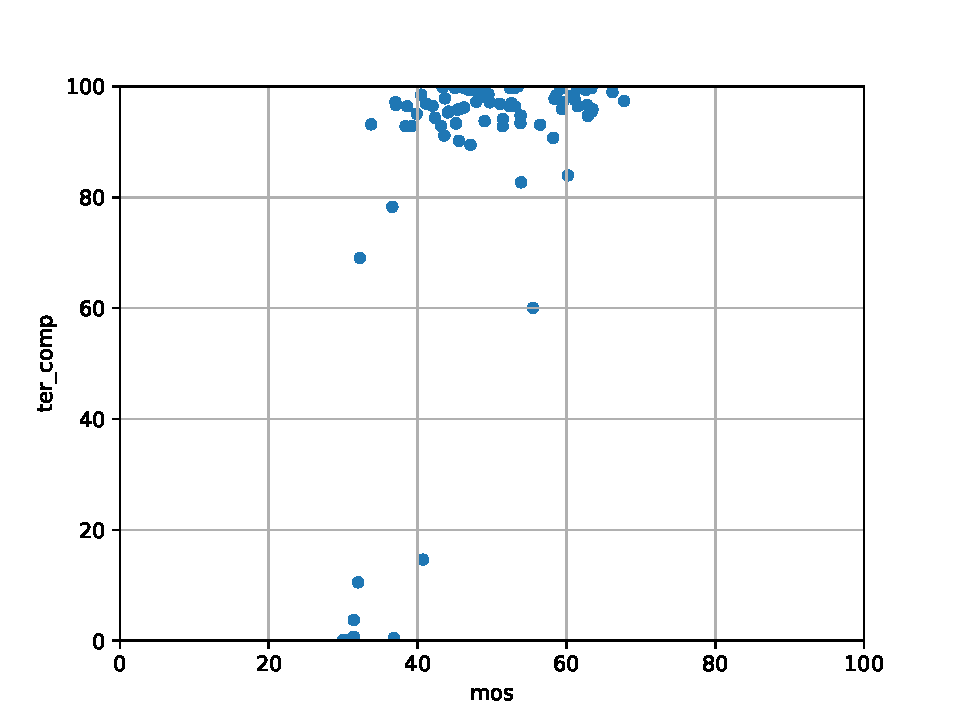
\includegraphics[width=\textwidth]{mosvster__456_22_29__1_4}
    \caption{\gls{cer} of a selection of distorted images compared to their reference image.}
    \label{fig:cer_vs_mos_456}
\end{figure}

\section{Codec Encoding}
\label{sec:dataset_codec}

In this section we first describe the extension of the dataset through encoding with the \gls{hevc} and \gls{vvc} codecs.
Additionally we detail the method we then use to compare the codecs by using the $\text{CER}_{\text{c}}$ and the \gls{bdrate}.

\subsection{High Efficiency Video Coding}
\label{subsec:hevc}

\gls{hevc} is a video codec.

\subsection{Versatile Video Coding}
\label{subsec:vvc}

\gls{vvc} is a video codec.

Furthermore, we encoded the images with the default and the \gls{scc} of the codecs to observe the difference.
The most important difference to the other distorted images is that there are no subjective scores available for these images.
However, the positive aspect is, that we can use more images for the comparison of the codecs, as we do not need to look out for objects overshadowing the text in the subjective scores.
The images used for the experiments with the codecs have the ID's $[1, 2, 3, 4, 5, 6, 7, 8, 9, 11, 12, 13, 15, 16, 18, 19, 20, 21, 22, 23, 24, 25, 27, 29]$.
For images encoded with these codecs the $\text{CER}_{\text{c}}$ can be calculated after predicting the text with the \gls{ocr} algorithms.

\begin{figure}
    \centering
    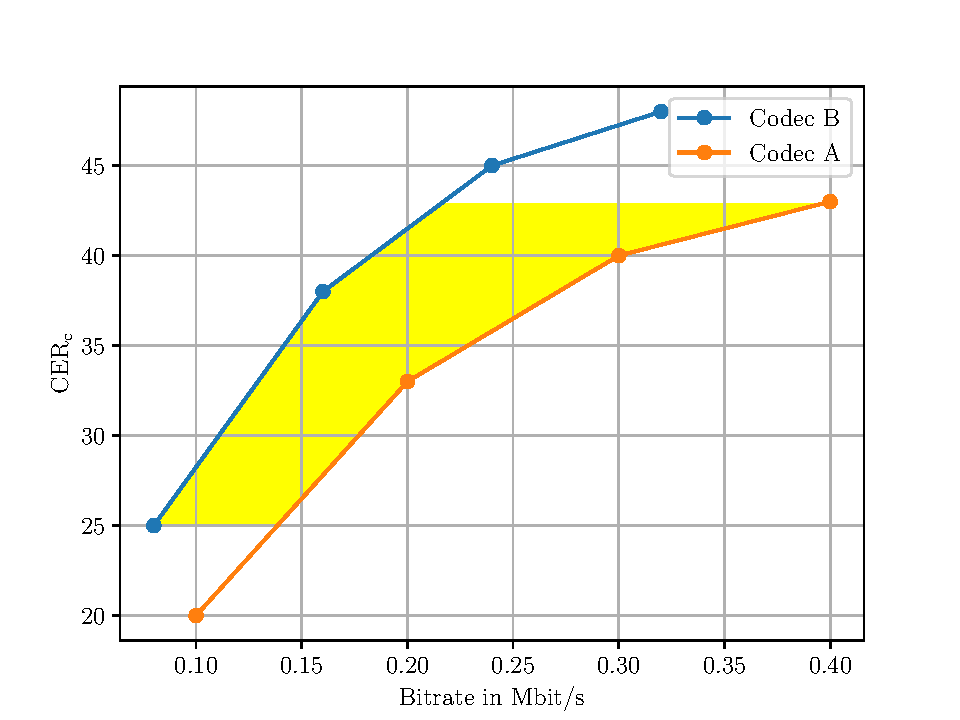
\includegraphics[width=\textwidth]{../../exp/bjontegaard_example.pdf}
    \caption{Example of the \gls{bdrate} calculation with dummy values. Adapted from \cite{bdrate_beyond_2022}}
    \label{fig:bdrate_example}
\end{figure}

Those $\text{CER}_{\text{c}}$ values can be plotted against the bitrate of the encoded images, see \autoref{fig:bdrate_example} for an example.
The different qualities can be denoted by $\text{i}$ and the different codecs by $\text{k}$.
In our case the qualities describe the \glspl{qp} values $[35, 40, 45, 50]$ and the codecs are $[\text{HM}, \text{VTM}]$.
- deviating from VVC common test conditions, due to lack of changes in the CER for lower QP values
Thus the points can be denoted as $\left(R_{\text{k,i}}, M_{\text{k,i}}\right)$ with $R_{\text{k,i}}$ being the bitrate and $D_{\text{k,i}}$ being the metric, in our case the $\text{CER}_{\text{c}}$.
Later, those points are averaged over all images to get the average bitrate and the average $\text{CER}_{\text{c}}$ for each codec.
The following section describes the calculation of the \gls{bdrate}, which can quantify the difference between the two curves of the codecs.

\subsection{Bjøntegaard Delta Rate}
\label{subsec:bdrate}

The \gls{bdrate} \cite{bdrate_original_2001}\cite{bdrate_beyond_2022} is defined as the average difference between two curves of the codecs to compare.
The first curve is the reference curve and the second the test curve.
The $R_{\text{k,i}}$ values are first converted to the log scale to not bias the results towards the higher bitrates with

\begin{equation}
    r_{\text{k,i}} = \log_{10}\left(R_{\text{k,i}}\right).
    \label{eq:log_scale}
\end{equation}

Those values in combination with the $\text{CER}_{\text{c}}$ values are then used as anchor points for a interpolation with a third order polynomial.
The resulting functions are denoted by $\hat{r}_{\text{k}}$, respectively.
The interpolation results in two curves, one for each codec, that pass through all anchor points.

Finally the \gls{bdrate} can be denoted as $\Delta R$ and is calculated by the integral of the difference between the two curves.
First, we need to define the lower and upper bound of the integral as follows

\begin{equation}
    \begin{aligned}
        M_{\text{low}} = \max\left(M_{\text{A},1}, M_{\text{B},1}\right) \\
        M_{\text{high}} = \min\left(M_{\text{A},4}, M_{\text{B},4}\right).
    \end{aligned}
    \label{eq:bounds}
\end{equation}

The bounds are just the maximum of the lowest quality points and the minimum of the highest quality points and can be seen in \autoref{fig:bdrate_example}.

\begin{equation}
    \Delta R = 10^{\frac{1}{M_{\text{low}}-M_{\text{high}}} \int_{M_{\text{low}}}^{M_{\text{high}}} \hat{r}_{\text{B}}(M) - \hat{r}_{\text{A}}(M) \text{d}M} - 1.
    \label{eq:bdrate}
\end{equation}

This value describes the average difference between the two curves in percent.
This enables us to compare two codecs.
Additionally we can calculate the same value, but with the $\text{CER}_{\text{c}}$ in relation to the ground truth instead of the reference.
These two values can then be compared to see if using the \gls{ocr} algorithms as a reference is a good approximation of the difference between codecs.
If the difference between the two values is small, then the approximation is good and we would not need a ground truth to evaluate new codecs.

To summarize, the original dataset has a \gls{mos} for each image with various distortions.
We are expanding the dataset by encoding the images with the \gls{hevc} and \gls{vvc} codecs.
The $\Delta R$ can then be calculated to compare two codecs and evaluate if the \gls{ocr} algorithms can be used as a approximate \gls{gt} for the \gls{bdrate} calculation.
